\resizebox{!}{5cm}{
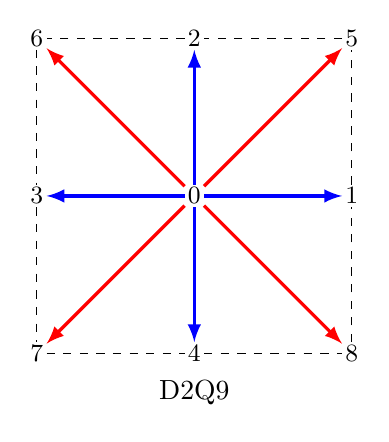
\begin{tikzpicture}[scale=1.0]
\begin{small}
\def\vscale{2.0};

\coordinate (C0) at (0,0);
\coordinate (C1) at (\vscale,0);
\coordinate (C2) at (0,\vscale);
\coordinate (C3) at (-\vscale,0);
\coordinate (C4) at (0,-\vscale);
\coordinate (C5) at (\vscale,\vscale);
\coordinate (C6) at (-\vscale,\vscale);
\coordinate (C7) at (-\vscale,-\vscale);
\coordinate (C8) at (\vscale,-\vscale);
%

%
\foreach \p in {0,1,...,8} {
	%\shadedraw (C\p) node (D\p) [circle,fill=gray!20,draw=black,shade,opacity=0.7]{\p};
	\draw (C\p) node[inner sep=1pt] (D\p){\p};
};
\draw[dashed] (D8)--(D1);
\draw[dashed] (D1)--(D5);
\draw[dashed] (D5)--(D2);
\draw[dashed] (D2)--(D6);
\draw[dashed] (D6)--(D3);
\draw[dashed] (D3)--(D7);
\draw[dashed] (D7)--(D4);
\draw[dashed] (D4)--(D8);

%\def\arrowcolors{{blue,blue,blue,blue,red,red,red,red}}
%\foreach \p in {1,2,...,8} {
\foreach \c [count = \p] in {blue,blue,blue,blue,red,red,red,red}{
	%\draw[->,thick] (D0)--(D\p);
	\draw[-latex,very thick,\c] (D0)--(D\p);
};
\end{small}
\coordinate (T) at (0,-2.5);
\draw (T) node{D2Q9};

\end{tikzpicture}
}
